%----------------------------------------------------------------------------------------------------------
% Slide 48

\begin{frame}
  \myheading{Module 6.7 : PCA : Practical Example}
\end{frame}

%----------------------------------------------------------------------------------------------------------
% Slide 49
\begin{frame}
  \begin{columns}
    \column{0.4\textwidth}<1->
    \begin{overlayarea}{\textwidth}{\textheight}
      \begin{minipage}[t]{0.15\textwidth}
        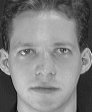
\includegraphics[width=\textwidth]{images/celebrity_images/s1_1.jpg}
      \end{minipage}
      \begin{minipage}[t]{0.15\textwidth}
        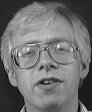
\includegraphics[width=\textwidth]{images/celebrity_images/s2_1.jpg}
      \end{minipage}
      \begin{minipage}[t]{0.15\textwidth}
        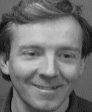
\includegraphics[width=\textwidth]{images/celebrity_images/s3_1.jpg}
      \end{minipage}
      \begin{minipage}[t]{0.15\textwidth}
        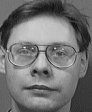
\includegraphics[width=\textwidth]{images/celebrity_images/s4_1.jpg}
      \end{minipage}

      \begin{minipage}[t]{0.15\textwidth}
        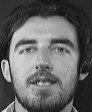
\includegraphics[width=\textwidth]{images/celebrity_images/s11_1.jpg}
      \end{minipage}
      \begin{minipage}[t]{0.15\textwidth}
        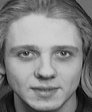
\includegraphics[width=\textwidth]{images/celebrity_images/s12_1.jpg}
      \end{minipage}
      \begin{minipage}[t]{0.15\textwidth}
        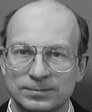
\includegraphics[width=\textwidth]{images/celebrity_images/s13_1.jpg}
      \end{minipage}
      \begin{minipage}[t]{0.15\textwidth}
        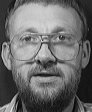
\includegraphics[width=\textwidth]{images/celebrity_images/s14_1.jpg}
      \end{minipage}

      \begin{minipage}[t]{0.15\textwidth}
        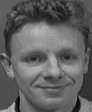
\includegraphics[width=\textwidth]{images/celebrity_images/s21_1.jpg}
      \end{minipage}
      \begin{minipage}[t]{0.15\textwidth}
        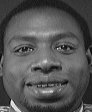
\includegraphics[width=\textwidth]{images/celebrity_images/s22_1.jpg}
      \end{minipage}
      \begin{minipage}[t]{0.15\textwidth}
        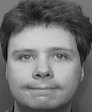
\includegraphics[width=\textwidth]{images/celebrity_images/s23_1.jpg}
      \end{minipage}
      \begin{minipage}[t]{0.15\textwidth}
        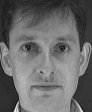
\includegraphics[width=\textwidth]{images/celebrity_images/s24_1.jpg}
      \end{minipage}

      \begin{minipage}[t]{0.15\textwidth}
        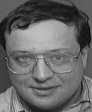
\includegraphics[width=\textwidth]{images/celebrity_images/s31_1.jpg}
      \end{minipage}
      \begin{minipage}[t]{0.15\textwidth}
        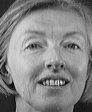
\includegraphics[width=\textwidth]{images/celebrity_images/s32_1.jpg}
      \end{minipage}
      \begin{minipage}[t]{0.15\textwidth}
        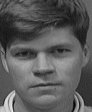
\includegraphics[width=\textwidth]{images/celebrity_images/s33_1.jpg}
      \end{minipage}
      \begin{minipage}[t]{0.15\textwidth}
        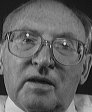
\includegraphics[width=\textwidth]{images/celebrity_images/s34_1.jpg}
      \end{minipage}
    \end{overlayarea}

    \column{0.6\textwidth}<1->
    \begin{overlayarea}{\textwidth}{\textheight}
      \begin{itemize}\justifying
        \item<1-> Consider we are given a large number of images of human faces (say, $m$ images)
        \item<2-> Each image is $100 \times 100$ [10K dimensions]
        \item<3-> We would like to represent and store the images using much fewer dimensions (around 50-200)
        \item<4-> We construct a matrix $X \in \mathbb{R}^{m \times 10K}$
        \item<5-> Each row of the matrix corresponds to 1 image
        \item<6-> Each image is represented using 10K dimensions
      \end{itemize}
    \end{overlayarea}
  \end{columns}
\end{frame}

%----------------------------------------------------------------------------------------------------------
% Slide 50
\begin{frame}
  \begin{columns}
    \column{0.4\textwidth}<1->
    \begin{overlayarea}{\textwidth}{\textheight}
      \onslide<6->{
        \begin{minipage}[t]{0.15\textwidth}
          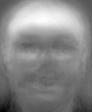
\includegraphics[width=\textwidth]{images/eig_docked_image/eig_1.jpeg}
        \end{minipage}
        \begin{minipage}[t]{0.15\textwidth}
          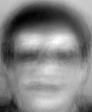
\includegraphics[width=\textwidth]{images/eig_docked_image/eig_2.jpeg}
        \end{minipage}
        \begin{minipage}[t]{0.15\textwidth}
          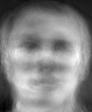
\includegraphics[width=\textwidth]{images/eig_docked_image/eig_3.jpeg}
        \end{minipage}
        \begin{minipage}[t]{0.15\textwidth}
          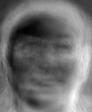
\includegraphics[width=\textwidth]{images/eig_docked_image/eig_4.jpeg}
        \end{minipage}

        \begin{minipage}[t]{0.15\textwidth}
          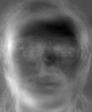
\includegraphics[width=\textwidth]{images/eig_docked_image/eig_5.jpeg}
        \end{minipage}
        \begin{minipage}[t]{0.15\textwidth}
          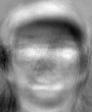
\includegraphics[width=\textwidth]{images/eig_docked_image/eig_6.jpeg}
        \end{minipage}
        \begin{minipage}[t]{0.15\textwidth}
          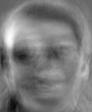
\includegraphics[width=\textwidth]{images/eig_docked_image/eig_7.jpeg}
        \end{minipage}
        \begin{minipage}[t]{0.15\textwidth}
          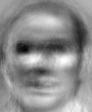
\includegraphics[width=\textwidth]{images/eig_docked_image/eig_8.jpeg}
        \end{minipage}

        \begin{minipage}[t]{0.15\textwidth}
          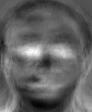
\includegraphics[width=\textwidth]{images/eig_docked_image/eig_9.jpeg}
        \end{minipage}
        \begin{minipage}[t]{0.15\textwidth}
          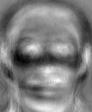
\includegraphics[width=\textwidth]{images/eig_docked_image/eig_10.jpeg}
        \end{minipage}
        \begin{minipage}[t]{0.15\textwidth}
          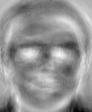
\includegraphics[width=\textwidth]{images/eig_docked_image/eig_11.jpeg}
        \end{minipage}
        \begin{minipage}[t]{0.15\textwidth}
          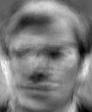
\includegraphics[width=\textwidth]{images/eig_docked_image/eig_12.jpeg}
        \end{minipage}

        \begin{minipage}[t]{0.15\textwidth}
          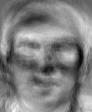
\includegraphics[width=\textwidth]{images/eig_docked_image/eig_13.jpeg}
        \end{minipage}
        \begin{minipage}[t]{0.15\textwidth}
          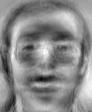
\includegraphics[width=\textwidth]{images/eig_docked_image/eig_14.jpeg}
        \end{minipage}
        \begin{minipage}[t]{0.15\textwidth}
          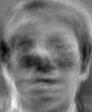
\includegraphics[width=\textwidth]{images/eig_docked_image/eig_15.jpeg}
        \end{minipage}
        \begin{minipage}[t]{0.15\textwidth}
          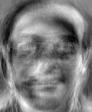
\includegraphics[width=\textwidth]{images/eig_docked_image/eig_16.jpeg}
        \end{minipage}
      }
    \end{overlayarea}

    \column{0.6\textwidth}<1->
    \begin{overlayarea}{\textwidth}{\textheight}
      \begin{itemize}\justifying
        \item<1-> $X \in \mathbb{R}^{m \times 10K}$ (as explained on the previous slide)
        \item<2-> We retain the top 100 dimensions corresponding to the top 100 eigen vectors of $X^T X$
        \item<3-> Note that $X^T X$ is a $n \times n$ matrix so its eigen vectors will be $n$ dimensional ($n=10K$ in this case)
        \item<4-> We can convert each eigen vector into a $100 \times 100$ matrix and treat it as an image
        \item<5-> Let's see what we get
        \item<6-> What we have plotted here are the first 16 eigen vectors of $X^T X$ (basically, treating each 10K dimensional eigen vector as a 100 $\times$ 100 dimensional image)

      \end{itemize}
    \end{overlayarea}
  \end{columns}
\end{frame}

%----------------------------------------------------------------------------------------------------------
% Slide 51
\begin{frame}
  \begin{columns}
    \column{0.5\textwidth}<1->
    \begin{overlayarea}{\textwidth}{\textheight}
      %\includegraphics[width=4cm]{images/recons_image_1/recons_1.jpg}
      %\begin{table}[]
      %\begin{tabular}{cccc}
      %\includegraphics[width=4cm]{images/recons_image_1/recons_1.jpg} & \includegraphics[width=4cm]{images/recons_image_1/recons_2.jpg} & \includegraphics[width=4cm]{images/recons_image_1/recons_5.jpg} & \includegraphics[width=4cm]{images/recons_image_1/recons_10.jpg} \\
      %\includegraphics[width=4cm]{images/recons_image_1/recons_20.jpg} & \includegraphics[width=4cm]{images/recons_image_1/recons_25.jpg}  & \includegraphics[width=4cm]{images/recons_image_1/recons_50.jpg} & \includegraphics[width=4cm]{images/recons_image_1/recons_80.jpg} \\
      %\includegraphics[width=4cm]{images/recons_image_1/recons_100.jpg} & \includegraphics[width=4cm]{images/recons_image_1/recons_125.jpg} & \includegraphics[width=4cm]{images/recons_image_1/recons_175.jpg} & \includegraphics[width=4cm]{images/recons_image_1/recons_200.jpg} \\
      %\includegraphics[width=4cm]{images/recons_image_1/recons_250.jpg} & \includegraphics[width=4cm]{images/recons_image_1/recons_275.jpg} & \includegraphics[width=4cm]{images/recons_image_1/recons_325.jpg} & \includegraphics[width=4cm]{images/recons_image_1/recons_400.jpg}
      %\end{tabular}
      %\end{table}
      \includegraphics<2->[width=0.15\textwidth]{images/celebrity_images/s1_1.jpg}

      \begin{minipage}[t]{0.15\textwidth}
        \visible<3->{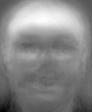
\includegraphics[width=\textwidth]{images/recons_images/recons_top_1.jpeg}}
      \end{minipage}
      \begin{minipage}[t]{0.15\textwidth}
        \visible<4->{\includegraphics[width=\textwidth]{images/recons_images/recons_top_2.jpeg}}
      \end{minipage}
      \begin{minipage}[t]{0.15\textwidth}
        \visible<5->{\includegraphics[width=\textwidth]{images/recons_images/recons_top_5.jpeg}}
      \end{minipage}
      \begin{minipage}[t]{0.15\textwidth}
        \visible<5->{\includegraphics[width=\textwidth]{images/recons_images/recons_top_10.jpeg}}
      \end{minipage}

      \begin{minipage}[t]{0.15\textwidth}
        \visible<6->{\includegraphics[width=\textwidth]{images/recons_images/recons_top_20.jpeg}}
      \end{minipage}
      \begin{minipage}[t]{0.15\textwidth}
        \visible<6->{\includegraphics[width=\textwidth]{images/recons_images/recons_top_25.jpeg}}
      \end{minipage}
      \begin{minipage}[t]{0.15\textwidth}
        \visible<6->{\includegraphics[width=\textwidth]{images/recons_images/recons_top_50.jpeg}}
      \end{minipage}
      \begin{minipage}[t]{0.15\textwidth}
        \visible<6->{\includegraphics[width=\textwidth]{images/recons_images/recons_top_80.jpeg}}
      \end{minipage}

      \begin{minipage}[t]{0.15\textwidth}
        \visible<7->{\includegraphics[width=\textwidth]{images/recons_images/recons_top_100.jpeg}}
      \end{minipage}
      \begin{minipage}[t]{0.15\textwidth}
        \visible<7->{\includegraphics[width=\textwidth]{images/recons_images/recons_top_125.jpeg}}
      \end{minipage}
      \begin{minipage}[t]{0.15\textwidth}
        \visible<7->{\includegraphics[width=\textwidth]{images/recons_images/recons_top_175.jpeg}}
      \end{minipage}
      \begin{minipage}[t]{0.15\textwidth}
        \visible<7->{\includegraphics[width=\textwidth]{images/recons_images/recons_top_200.jpeg}}
      \end{minipage}

      \begin{minipage}[t]{0.15\textwidth}
        \visible<8->{\includegraphics[width=\textwidth]{images/recons_images/recons_top_250.jpeg}}
      \end{minipage}
      \begin{minipage}[t]{0.15\textwidth}
        \visible<8->{\includegraphics[width=\textwidth]{images/recons_images/recons_top_275.jpeg}}
      \end{minipage}
      \begin{minipage}[t]{0.15\textwidth}
        \visible<8->{\includegraphics[width=\textwidth]{images/recons_images/recons_top_325.jpeg}}
      \end{minipage}
      \begin{minipage}[t]{0.15\textwidth}
        \visible<8->{\includegraphics[width=\textwidth]{images/recons_images/recons_top_400.jpeg}}
      \end{minipage}
      \begin{align*}
        \only<3>{\sum_{i=1}^{1} \alpha_{1i} p_i}
        \only<4>{\sum_{i=1}^{2} \alpha_{1i} p_i}
        \only<5>{\sum_{i=1}^{4} \alpha_{1i} p_i}
        \only<6>{\sum_{i=1}^{8} \alpha_{1i} p_i}
        \only<7>{\sum_{i=1}^{12} \alpha_{1i} p_i}
        \only<8->{\sum_{i=1}^{16} \alpha_{1i} p_i}
      \end{align*}
    \end{overlayarea}

    \column{0.5\textwidth}<1->
    \begin{overlayarea}{\textwidth}{\textheight}
      \begin{itemize}\justifying
        \item<1-> These images are called eigenfaces and form a basis for representing any face in our database
        \item<2-> In other words, we can now represent a given image (face) as a linear combination of these eigen faces
        \item<9-> In practice, we just need to store $p_1,p_2,\cdots,p_{k}$ (one time storage)
        \item<10-> Then for each image $i$ we just need to store the scalar values $\alpha_{i1},\alpha_{i2},\cdots,\alpha_{ik}$
        \item<11-> This significantly reduces the storage cost without much loss in image quality
              %\item<4-> Let us get some more perspective on eigen vectors before moving ahead
      \end{itemize}
    \end{overlayarea}
  \end{columns}
\end{frame}